%!TEX root = ../../dissertation.tex
%%%%%%%%%%%%%%%%%%%%%%%%%%%%%%%%%%%%%%%%%%%%%%%%%%%%%%%%%%%%%%%%%%%%%%%%%%%%%%%%
\section{Survey of 3G/4G Evaluation and Simulation Frameworks}

While there are some active measurement studies specifically targeted at reliable streaming in mobile networks, e.g., \cite{Muller:2012:EDA:2151677.2151686}, most rely either on fixed networks or simulations.


Simulation frameworks are especially important for mobile networks, as acquiring packet-level traces and information about every node in an actual commercially operating cellular network is nigh impossible due to the users' privacy and the provider's business concerns.

Therefore, it would be very desirable to find an existing framework, that covers all important aspect in 3G or 4G mobile networks.

Most 3G/4G simulators only concern themselves with he physical radio link, completely neglect all other network paths, especially the core and all control plane signaling interactions.

Interestingly, the situation is even worse for \gls{UMTS} despite being significantly older.

The following list summarizes a number of simulators.

\begin{itemize}

	\item Radio system level UMTS for ns-2
\url{http://net.infocom.uniroma1.it/reti_files/reti_downloads.htm}
outdated, not up-to-date to newest standards

	\item \url{http://www.valid8.com/UMTS_Core_Network_Simulator.html} Not publicly available and commercial
also seems to focus on the circuit switched domain

	\item \url{http://seacorn.cs.ucy.ac.cy/eumtssim/}
\cite{vranjevs2011use}
Seacorn UMTS simulator (rather patches to ns-2), no public access
does not include any of the core network's protocols or procedures
but is also based on outdated specs and not actively maintained

	\item Only commercial: UMTS model in OPNET (now: Riverbed Modeler)
\url{http://www.riverbed.com/products/performance-management-control/network-performance-management/network-simulation.html}
again radio and user plane focused 

	\item Matlab-based radio link system-level sim
\url{http://www.nt.tuwien.ac.at/research/mobile-communications/lte-simulators/}

	\item LTE-Sim
Simulating LTE Cellular Systems: An Open-Source Framework \cite{5634134}
\url{http://telematics.poliba.it/index.php/en/lte-sim}
simulates some nodes (UE, eNB, MME) and only a limited selection of involved protocols (PDCP, RLC, very basic RRC)
very limited for network/transport layer protocols (only basic ip, tcp not even implemented), rudimentary implementation not even close to reality

	\item Omnet++ \url{http://www.omnetpp.org/}
with SimuLTE framework https://github.com/inet-framework/simulte
only user plane (but also user plane core nodes SGW/PGW)
comparable level to ns-3

	\item ns-3
\gls{LTE}-\gls{EPC} Network Simulator (LENA)\cite{Baldo:2013:OSM:2507924.2507940} 
\url{http://networks.cttc.es/mobile-networks/software-tools/lena/}
\url{http://www.nsnam.org/docs/release/3.20/doxygen/group__lte.html}
\url{http://www.nsnam.org/docs/release/3.20/models/html/lte.html}
Most complete of all open source simulation approaches, but still only very rudimentary in the core and signaling
but combined with ns-3 offers almost complete representation of a vanilla network and transport level network stack
Can also use Network Simulation Cradle (NSC) \url{http://research.wand.net.nz/software/nsc.php}
to incorporate the actual Linux TCP/IP stack
however: only 2.6.26 (very old!)
and less instrumentation/logging available for this stack

\end{itemize}



%%%%%%%%%%%%%%%%%%%%%%%%%%%%%%%%%%%%%%%%%%%%%%%%%%%%%%%%%%%%%%%%%%%%%%%%%%%%%%%%
\section{Combined Simulating Streaming Traffic Characteristics in ns-3}
\label{c6:mobilestreamingtestbed}


Different Approaches



Implement a Reliable Streaming Traffic Generator ns-3 Application and a streaming receiver client application.

Describe Streaming Simulation Model and Variables

Describe ns-3/LENA implementation

 Use LENA to transport streams


 test case 1: adaptability of diverse reliable video streaming to LTE and mobile networks, by altering latency, loss, bandwidth

 test case 2a (future): influence of mobility effects on reliable streaming
 test case 2b (future): effect of cross-layer information in mobility case



\begin{figure}[htb]
\centering
\includegraphics[width=0.6\textwidth]{images/streaming-simulation.pdf}
\caption{\gls{LTE} reliable streaming simulation testebd.}
\label{c5:fig:streaming-simulation}
\end{figure}


%%
\subsection{Simulation/Emulation Hybrid}


Use introduced streaming evaluation approaches in a mobile network environment

But do not want to use real network, as conditions are hard to manage and reproduce.

comparable to the initial (simple) network emulation used in the measurement framework in Section~\ref{c3:measurements} using static values
here it acts as a dynamic network emulator, delaying packets based on its pass-through time through the network, while also adding packet loss.

Therefore, use an emulated network provided by the ns-3 network simulator. But transmit real traffic through it, i.e., use it as an emulator and bridges. \ref{c5:fig:streaming-simulation} \ref{c5:fig:streaming-hybrid}


\begin{figure}[htb]
\centering
\includegraphics[width=\textwidth]{images/streaming-hybrid.pdf}
\caption{Future testbed iteration: hybrid of ns-3 LTE simulation and actual or emulated streaming client and server bridged to it.}
\label{c5:fig:streaming-hybrid}
\end{figure}



\begin{figure}[htb]
\centering
\includegraphics[width=1.0\textwidth]{images/R-ltesim-plotbuffer-time.pdf}
\caption{R-ltesim-plotbuffer-time.pdf}
\label{c5:fig:ltesim-plotbuffer-time}
\end{figure}


\begin{figure}[htb]
\centering
\includegraphics[width=1.0\textwidth]{images/R-ltesim-bwseries-numstalls.pdf}
\caption{R-ltesim-bwseries-numstalls.pdf}
\label{c5:fig:ltesim-bwseries-numstalls}
\end{figure}

\begin{figure}[htb]
\centering
\includegraphics[width=1.0\textwidth]{images/R-ltesim-bwseries-stallduration.pdf}
\caption{R-ltesim-bwseries-stallduration.pdf}
\label{c5:fig:ltesim-bwseries-stallduration}
\end{figure}

\begin{figure}[htb]
\centering
\includegraphics[width=1.0\textwidth]{images/R-ltesim-latencyseries-numstalls.pdf}
\caption{R-ltesim-latencyseries-numstalls.pdf}
\label{c5:fig:ltesim-latencyseries-numstalls}
\end{figure}

\begin{figure}[htb]
\centering
\includegraphics[width=1.0\textwidth]{images/R-ltesim-latencyseries-stallduration.pdf}
\caption{R-ltesim-latencyseries-stallduration.pdf}
\label{c5:fig:ltesim-latencyseries-stallduration}
\end{figure}


% \begin{figure}[htb]
% \centering
% \includegraphics[width=\textwidth]{images/lte-testbed.pdf}
% \caption{\gls{LTE} Streaming Evaluation Setup and Action Plan}
% \label{fig:lte-testbed}
% \end{figure}


